\chapter{Implementation} \label{implementation}

For this project I decided to use the Rust programming language. It is a
performant, memory safe language that is similar to C++. Additionally, it has
very good parallel programming facilities and an extensive software ecosystem
that makes it ideal for this kind of project.

The implementation is a command line application that takes a source code file
as input and generates a 

The Rust code in the fern repository showcases a comprehensive implementation of
a language processing system, including lexical analysis, parsing, and possibly
semantic analysis and code generation. Here's an overview of the implementation
based on the provided Rust code files: Key Components:
Lexical Analysis (src/lexer.rs, src/grammar/lg.rs)

    Lexer Implementation: The lexer component is responsible for tokenizing
the input source code. It uses a set of rules defined in src/grammar/lg.rs to
match patterns in the input text and convert them into tokens. This process is
crucial for the parsing stage, as it simplifies the input by abstracting away
the textual representation into a series of tokens with assigned meanings.

Parsing (src/parser.rs, src/parsetree.rs)
    Parser and Parse Tree: The parser takes the tokens generated by the lexer
    and constructs a parse tree based on the grammar of the language being
    analyzed. This tree represents the syntactic structure of the input code.
    The implementation in src/parser.rs and src/parsetree.rs likely involves
    recursive descent parsing or another parsing technique to handle the
    language's grammar.

Semantic Analysis (src/analysis.rs)

    Analysis: After parsing, the src/analysis.rs file suggests that the code
performs some form of semantic analysis. This could involve checking variable
declarations before use, type checking, or other compile-time checks that ensure
the program's semantic correctness.

Intermediate Representation (src/ir.rs)

    Intermediate Representation (IR): The src/ir.rs file indicates the
generation of an intermediate representation of the code. IR is a lower-level
representation of the program that is easier for a compiler or interpreter to
optimize and translate into machine code or another target language.

Language Specific Implementations (src/eslang.rs, src/json.rs, src/fern.rs)

    Language Implementations: The repository includes specific implementations
for different languages or formats, such as a custom language (src/eslang.rs),
JSON (src/json.rs), and possibly "fern" itself (src/fern.rs). These files
contain the rules and logic for parsing and analyzing these specific languages.

Implementation Overview for Report:
In your report's implementation section, you could describe how the project
is structured around the core components of a compiler or interpreter: lexical
analysis, parsing, semantic analysis, and intermediate representation. Highlight
the modular design that allows for the processing of different languages, as
evidenced by the separate implementations for each language. Discuss the use of
Rust's powerful type system and ownership model to manage resources efficiently
and ensure memory safety throughout the compilation process.

You might also want to mention the use of external libraries (if any are used)
and how they integrate with the project's codebase to enhance functionality,
such as for parallel processing or handling complex data structures.

Finally, consider discussing the project's testing strategy, based on the
presence of tests/ and benches/ directories, to ensure the reliability and
performance of the language processing system.

Would you like more detailed information or assistance with another part of
your report?


\subsection{Generating the Operator Precedence Table}

\begin{listing}[H]
\begin{minted}[linenos]{text}
fn factorial[n: int] {
    if n == 0 {
        return 1;
    % } 

    return (n * factorial(n - 1));
}
\end{minted}
\caption{Factorial in the test language.}
\label{lst:factorial_example}
\end{listing}

\begin{listing}[H]
\begin{minted}[linenos]{json}
{
  "a": 100,
  "b": {
    "x": [
      100,
      "a"
    ]
  }
}
\end{minted}
\caption{Example of parsable JSON.}
\hrulefill
\label{lst:json_example}
\end{listing}

Section \ref{dependancies}
\newline \newline
Section \ref{structure}
\newline \newline
Section \ref{outputs_and_visualizations}
\newline \newline
Section \ref{debugging}

\section{Dependencies} \label{dependancies}
\section{Structure} \label{structure}
\subsection{Parsing Grammar Transformation} \label{parsing_grammar_transformation}
\section{Outputs and Visualizations} \label{outputs_and_visualizations}

\begin{figure}[t]
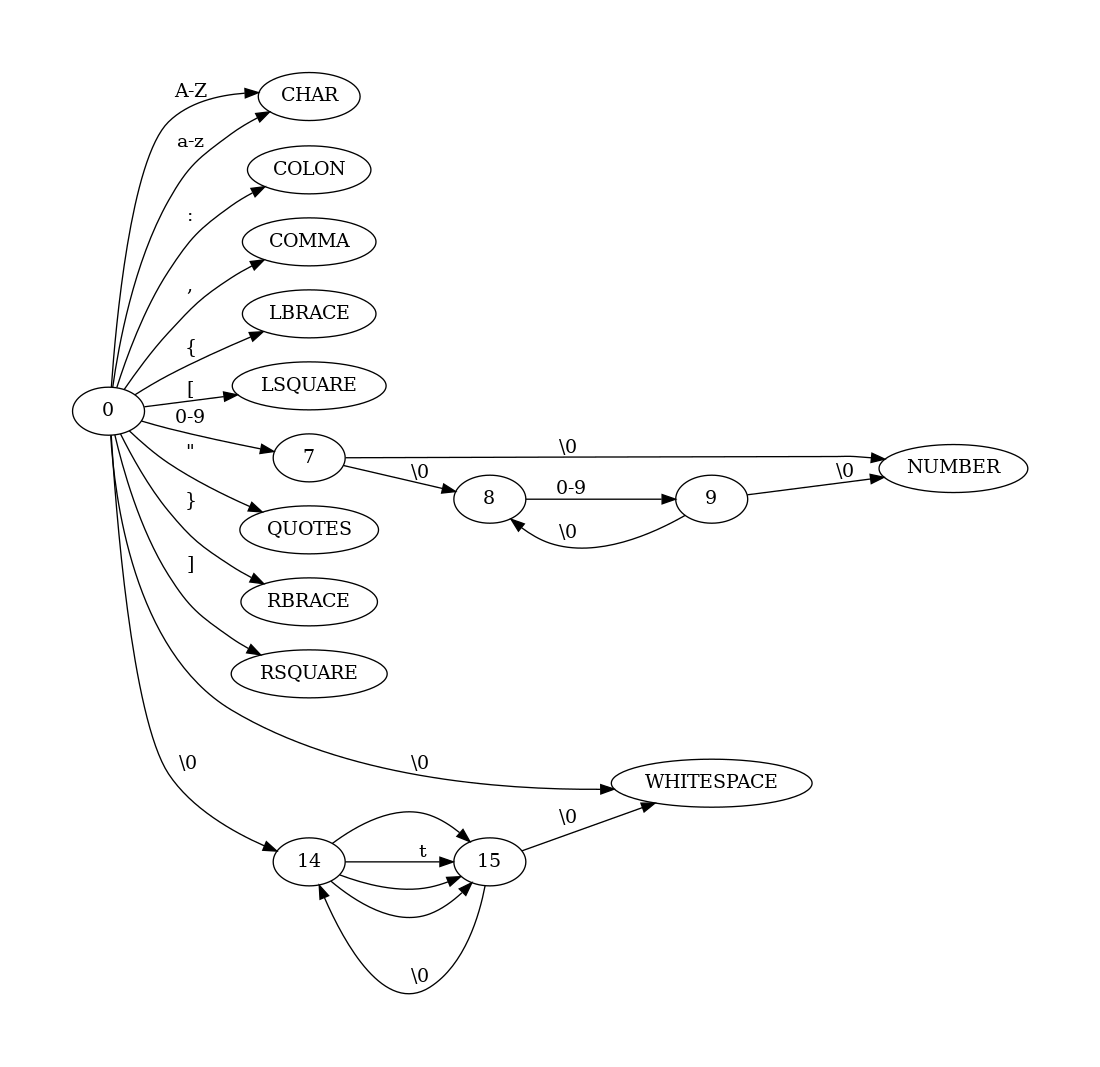
\includegraphics[width=\linewidth]{images/nfa.png}
\caption{NFA of the lexical grammar}
\label{fig:nfa}
\end{figure}

\begin{figure}[t]
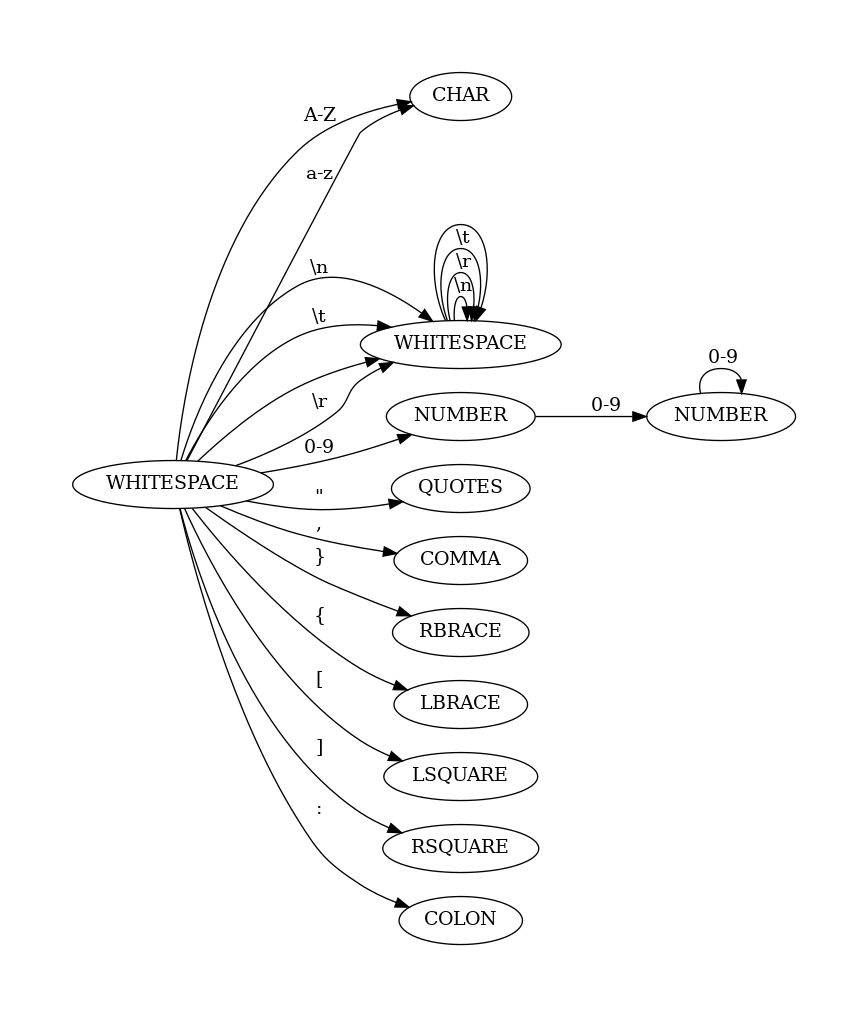
\includegraphics[width=\linewidth]{images/dfa.png}
\caption{DFA of the lexical grammar}
\label{fig:dfa}
\end{figure}

\begin{figure}[t]
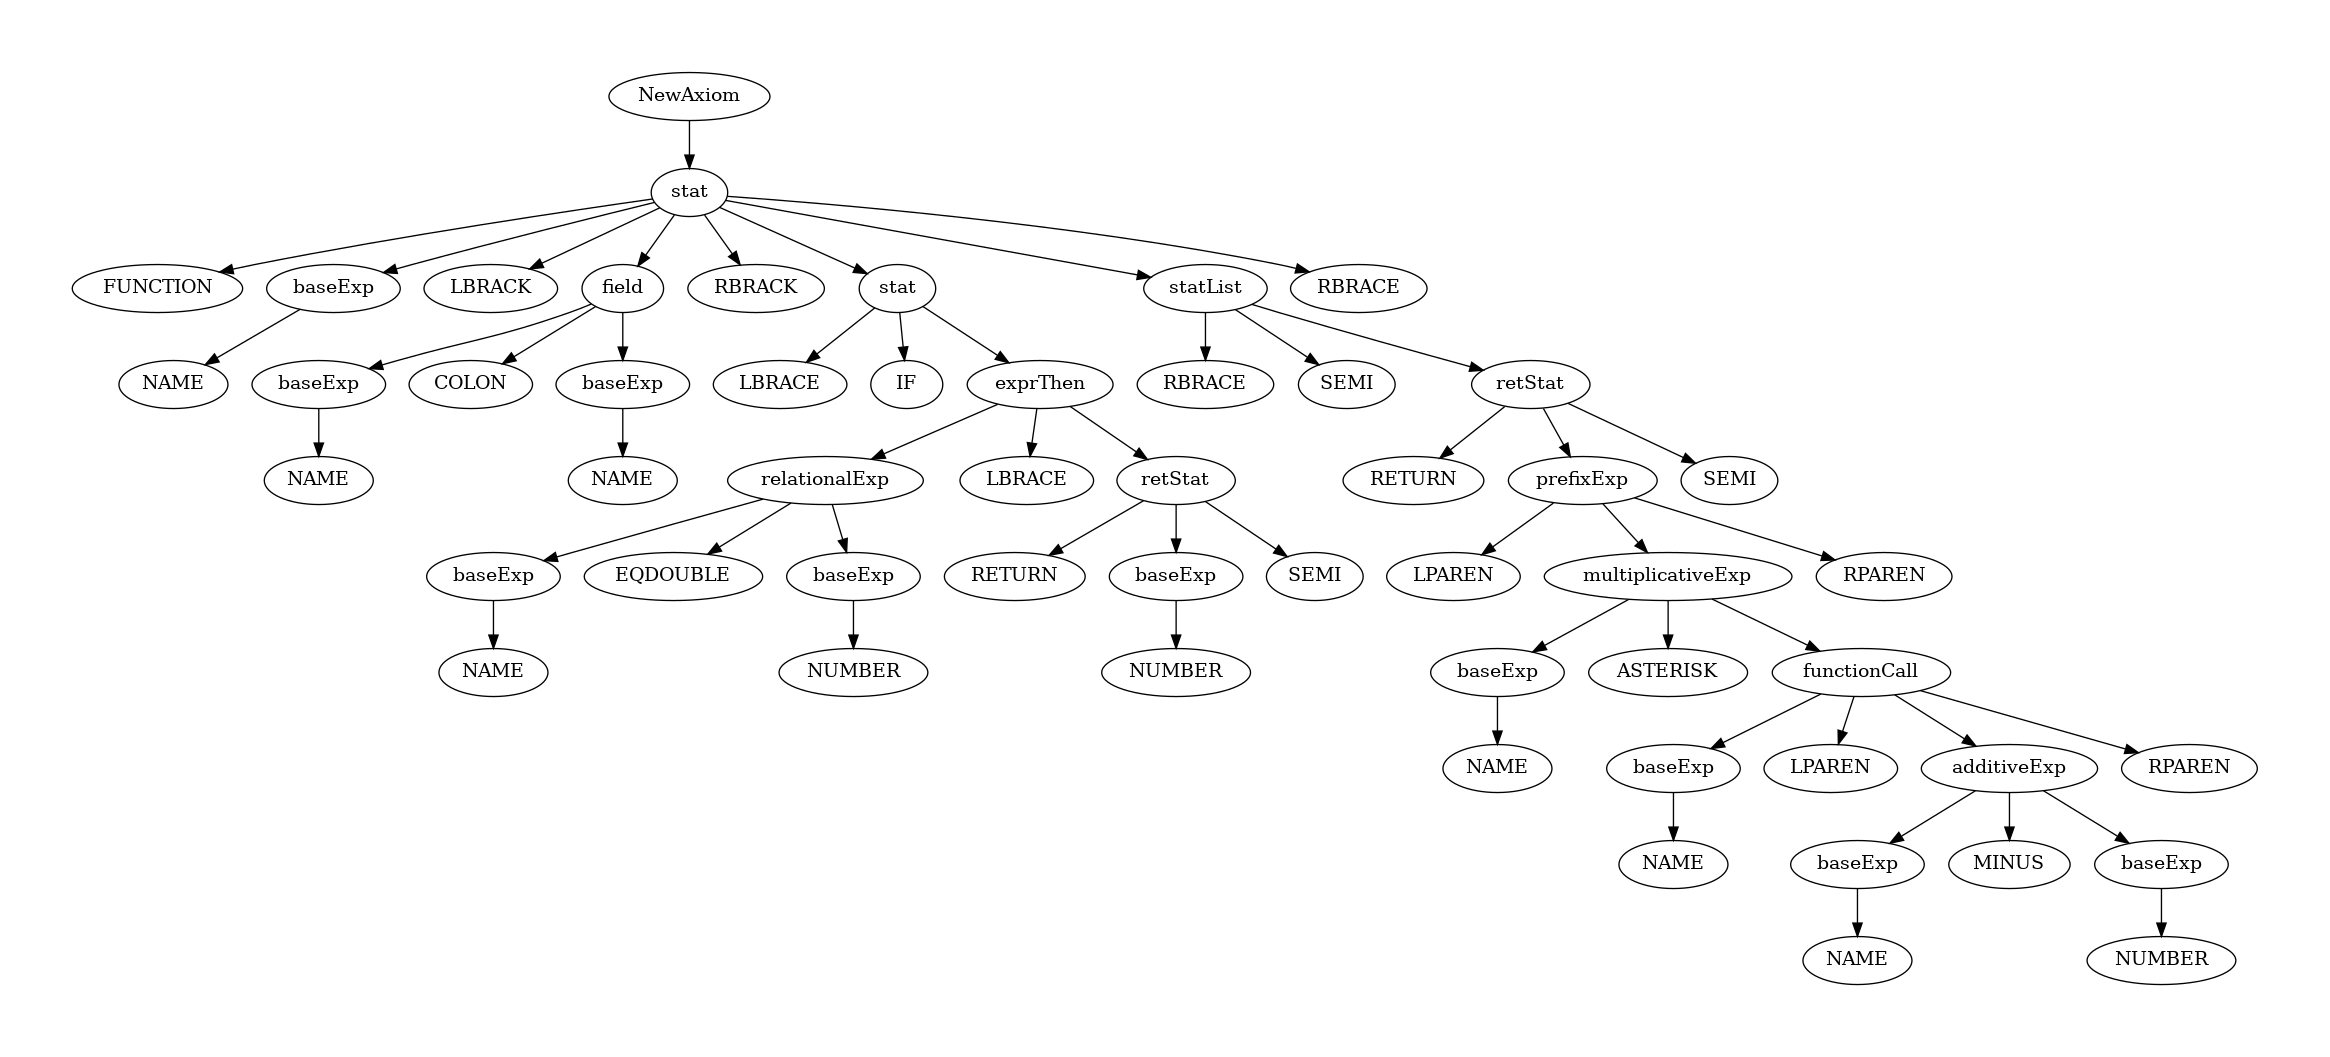
\includegraphics[width=\linewidth]{images/ptree.png}
\caption{Graphviz visualization of the parse tree.}
\label{fig:parse_tree}
\end{figure}

\section{Debugging} \label{debugging}
